\HeaderQuote{Read the directions and directly you will be directed in the right direction.}{Doorknob} 

\chapter{\Jsp\ Scheduling Problem}\label{ch:scheduling}
\FirstSentence{S}{cheduling problems}, which occur frequently in practice, are 
a category within combinatorial optimisation problems. 
A subclass of scheduling problems is \jsp\ (\JSP), which 
is widely studied in operations research. 
\JSP\ deals with the allocation of tasks of competing resources where its goal 
is to optimise one ore more objectives. 
\Jsp's analogy is from the manufacturing industry where a set of jobs are 
broken down into tasks that must be processed on several machines in a 
workshop. 
Furthermore, its formulation can be applied on a wide variety of practical 
problems in real-life applications which involve decision making. Therefore, 
its problem-solving capabilities have a high impact on many manufacturing 
organisations. % Gefa dæmi?

Deterministic \JSP\ is the most \emph{general} case for classical scheduling problems \citep{Jain99}. 
Many other scheduling problems can be reformulated as \JSP. 
For instance, the \textit{travelling salesman problem}\footnote{
    The travelling salesman problem (TSP) was formulated in the 1800s by the 
    mathematicians W.R. Hamilton and Thomas Kirkman \citep{graphtheory}. 
    The salesman has to visit a set of cities exactly once (i.e. Hamiltonian 
    path), with the objective of minimising the route, in terms of distance, 
    between them.}
 can be contrived as \JSP
\begin{enumerate*}[label={{}}]
    \item the salesman as a single machine in use
    \item the cities to be visited are the jobs to be processed
    \item distance is sequence dependent set-up time
\end{enumerate*}
The general form of~~\JSP\ assumes that each job can have its own 
distinctive flow pattern through the machines, which is independent of the 
other jobs. 
In the case where all jobs share the same permutation route, \jsp\ is reduced 
to a \fsp\ scheduling problem (\FSP) \citep{Guinet1998,Tay08}. 
Therefore, without loss of generality, this dissertation is structured around 
\JSP. 

\emph{Remark:} Throughout the dissertation the \FSP\ variation will \emph{not} 
be a commonly used permutation \fsp\ (P\FSP) from the 
literature,\footnote{\Cref{InRu12} wrongly states that it is used P\FSP\ problem
    instances, it was in fact \FSP.} 
which has the added constraints of not allowing any jobs to pass one another.
Here, the jobs have to be processed in the same machine order. However, 
machines do not necessarily need to process jobs in the same order, as is 
implied in P\FSP. For P\FSP\ the \citet{Manne60} model would be more 
appropriate, rather than the one described in the following 
\lcnamecref{jsp:MIP}.

\section{Mathematical formulation}\label{jsp:MIP}
\Jsp\ considered for this dissertation is when $n$ jobs, 
$\mathcal{J}=\{J_j\}_{j=1}^n$, are scheduled on a finite set, 
$\mathcal{M}=\{M_a\}_{a=1}^m$, of $m$ machines, subject to the constraint that 
each job $J_j$ must follow a predefined machine order (a chain of 
$m$ operations, $\vsigma_j=[\sigma_{j1},\sigma_{j2},\dotsc,\sigma_{jm}]$) and 
that a machine can handle at most one job at a time. 
The objective is to schedule jobs in such a manner as to minimise the maximum 
completion times for all tasks, which is also known as the makespan, 
$C_{\max}$. 

A common notation for scheduling problems \citep[cf. Chapter 2 in ][]{Pinedo08} 
is given by a triplet $\alpha|\beta|\gamma$, where 
\begin{enumerate*}[itemjoin*={, and finally}, label={{}}]
    \item $\alpha$ describes the machine environment
    \item $\beta$ details any additional processing characteristics and/or 
    constraints
    \item $\gamma$ lists the problem's objective
\end{enumerate*}
Hence our family of scheduling problems, i.e., a $m$ machine \JSP\ and \FSP\ 
w.r.t. minimising makespan, is $Jm||C_{\max}$ and $Fm||C_{\max}$, respectively. 
An additional constraint commonly considered are job release-dates and 
due-dates, and then the objective is generally minimising the maximum lateness, 
denoted $Jm|r_j,d_j|L_{\max}$. 
However, those shop-requirements will not be considered here. 

Henceforth, the index $j$ refers to a job $J_j\in\mathcal{J}$, while the index 
$a$ refers to a machine $M_a\in\mathcal{M}$. If a job requires a number of 
processing steps or operations, then the pair $(j,a)$ refers to the operation, 
i.e., processing the task of job $J_j$ on machine $M_a$. Moreover, index $k$ 
will denote the time step of the operation. Note that once an operation is 
started it must be completed uninterrupted, i.e., pre-emption is not allowed. 
Moreover, there are no sequence dependent set-up times.

For any given \JSP\ each job $J_j$ has an indivisible processing time (or 
cost) on machine $M_a$, $p_{ja}$, which is assumed to be integral and finite. 

The starting time of job $J_j$ on machine $M_a$ is denoted $x_s(j,a)$ and its 
completion or end time is denoted $x_e(j,a)$ where, 
\begin{equation}  x_e(j,a):=x_s(j,a)+p_{ja} \end{equation} 


Each job $J_j$ has a specified processing order through the machines, it is a 
permutation vector, $\vsigma_j$, of $\{1,..,m\}$, representing a job $J_j$ can 
be processed on $M_{\vsigma_j(a)}$ only after it has been completely processed 
on $M_{\vsigma_j(a-1)}$, i.e.,
\begin{equation}\label[ineq]{eq:permutation}
x_s(j,\vsigma_j(a)) \geq x_e(j,\vsigma_j(a-1)) 
\end{equation}
for all $J_j\in\mathcal{J}$ and $a\in\{2,..,m\}$. 
Note, that each job can have its own distinctive flow pattern through the 
machines, which is independent of the other jobs. However, in the case that all 
jobs share the same permutation route, \JSP\ is reduced to a \FSP.

The disjunctive condition that each machine can handle at most one job at a 
time is the following,
\begin{equation}\label[ineq]{eq:oneJobPerMac}
x_s(j,a) \geq x_e(j',a) \quad\textrm{or}\quad x_s(j',a) \geq x_e(j,a)  
\end{equation}
for all $J_j,J_{j'}\in\mathcal{J},\; J_j\neq J_{j'}$ and $M_a\in\mathcal{M}$. 

The objective function is to minimise its maximum completion times for all 
tasks, commonly referred to as the makespan, $C_{\max}$, which is defined as 
follows,
\begin{equation}
C_{\max} := \max\condset{x_e(j,\vsigma_j(m))}{J_j\in\mathcal{J}}.
\label{eq:makespan}
\end{equation} 
Clearly, w.r.t. minimum makespan, it is preferred that schedules are non-delay, 
i.e., the machines are not kept idle. The time in which machine $M_a$ is idle 
between consecutive jobs $J_j$ and $J_{j'}$ is called idle time, or slack,
\begin{equation} 
s(a,j):=x_s(j,a)-x_e(j',a) \label{eq:slack}
\end{equation}
where $J_j$ is the immediate successor of $J_{j'}$ on $M_a$. Although this is 
not a variable directly needed to construct a schedule for \JSP, it is a key 
attribute in order to measure the quality of the schedule. 

Note, from a job-oriented viewpoint, for a job already dispatched 
$J_j\in\mathcal{J}$ the corresponding set of machines already processed is 
$\mathcal{M}_j\subset\mathcal{M}$. Similarly from the machine-oriented 
viewpoint, $M_a\in\mathcal{M}$ with corresponding 
$\mathcal{J}_a\subset\mathcal{J}$. 

\section{Construction heuristics}\label{sec:CH}
Construction heuristics are designed in such a way that it limits the search 
space in a logical manner, preferably without excluding the true optimum. 
Here, the construction heuristic, $\Upsilon$, is to schedule the dispatches as 
closely together as possible, i.e., minimise the schedule's idle times. 
More specifically, once an operation $(j,a)$ has been chosen from the job-list, 
$\mathcal{L}$, by some dispatching rule, it can placed immediately after (but 
not prior) $x_e(j,\vsigma_j(a-1))$ on machine $M_a$ due to 
\cref{eq:permutation}.
However, to guarantee that \cref{eq:oneJobPerMac} is not violated, 
idle times $M_a$ are inspected, as they create a slot which in $J_j$ can 
occupy. Bearing in mind that $J_j$ release time is $x_e(j,\vsigma_j(a-1))$ one 
cannot implement \cref{eq:slack} directly, instead it has to be updated as 
follows,
\begin{equation}
\tilde{s}(a,j') := x_s(j'',a)-\max\{x_e(j',a),\;x_e(j,\vsigma_j(a-1))\} % 
%\textrm{ if } x_e(j,\vsigma_j(a-1)\geq x_e(j',a) 
\end{equation}
for all already dispatched jobs $J_{j'},J_{j''}\in \mathcal{J}_a$ where 
$J_{j''}$ is $J_{j'}$ successor on $M_a$. Since pre-emption is not allowed, the 
only applicable slots are whose idle time can process the entire operation, 
i.e.,
\begin{equation}
\tilde{S}_{ja} := \condset{J_{j'}\in \mathcal{J}_a}{\tilde{s}(a,j')\geq 
    p_{ja} }\label{eq:slots}.
\end{equation} 
There are several heuristic methods for selecting a slot from 
\cref{eq:slots}, e.g., if the main concern were to utilise the slot space, then 
choosing the slot with the smallest idle time would yield a closer-fitted 
schedule and leaving greater idle times undiminished for subsequent dispatches 
on $M_a$. However, dispatching $J_j$ in the first slot would result in its 
earliest possible release time, which would be beneficial for subsequent 
dispatches for $J_j$. Experiments favoured dispatching in the 
earliest slot,\footnote{Preliminary experiments of 500 \JSP\ instances where 
    inspected: First slot chosen could always achieve its known optimum by 
    implementing \cref{pseudo:constructJSP}, however, only $97\%$ of
    instances when choosing the smallest slot.} 
thus used throughout.

Note that the choice of slot is an intrinsic heuristic within $\Upsilon$.
The focus of this dissertation, however, is on learning the priority of the 
jobs on the job-list, for a fixed construction heuristic. 
Hence, there could be some problem instances in which the optimum makespan 
cannot be achieved, due to the limitations of $\Upsilon$ of not being properly 
able to differentiate between which slot from \cref{eq:slots} is the most 
effective.
Instead, hopefully, the learning algorithm will be able to spot these 
problematic situations, should they arise, by inspecting the schedule's 
features and translate that into the jobs' priorities.

\subsubsection*{Dispatching rules}

\emph{Dispatching rules} (DR) are an integral part of a construction 
heuristics, as it determines the priorities of the job-list, i.e., 
the jobs who still have operations unassigned. 
Starting with an empty schedule, and sequentially adding one operation (or 
task) at a time. Then, for each time step $k$, an operation is dispatched which 
has the highest priority of the 
job-list, \mbox{$\mathcal{L}^{(k)}\subset\mathcal{J}$}.
If there is a tie, some other priority measure is used. 
However, let's assume that ties are broken randomly. 
\Cref{pseudo:constructJSP} outlines the pseudo code for the entire dispatching 
process of a \JSP\ problem instance.

\clearpage
\begin{algorithm}
    \caption{Pseudo code for constructing a \JSP\ sequence using a dispatching 
    rule (DR) for a fixed construction heuristic (Y).} 
    \label{pseudo:constructJSP}
    \begin{algorithmic}[1]
        \Procedure{Constructing \JSP}{DR,Y}
        \State $\vchi \gets \emptyset$ current dispatching sequence  
        \Comment{initialization}
        \For{$k:=1~\textbf{to}~l=n\cdot m$} 
        \Comment{at each dispatch iteration}
        \ForAll{$J_j\in \mathcal{L}^{(k)}\subset \mathcal{J}$} 
        \Comment{inspect job-list}
        \State $I_j^{DR}\leftarrow \text{DR}\left([\vchi,j],Y\right)$ 
        \Comment{priority $J_j$}
        \EndFor
        \State $j^* \gets \argmax_{j\in \mathcal{L}^{(k)}}\{I_j^{DR}\}$ 
        \Comment{choose highest priority}
        \State $\chi_k \gets j^*$ 
        \Comment{dispatch $j^*$}
        \EndFor
        \State \Return $C_{max} \gets Y(\vchi)$ 
        \Comment{makespan and final schedule}
        \EndProcedure
    \end{algorithmic}
\end{algorithm}

Henceforth, we will adopt the following terminology: a \emph{sequence} will 
refer to the sequential ordering of the dispatches\footnote{Note, 
    only a sequence of $J_j$ is needed, since the corresponding $M_a$ can be 
    obtained by reading $\vsigma$.} 
of tasks to machines, namely, 
\begin{equation} \label{eq:vchi}
\vchi = \big\{\chi_k\big\}_{k=1}^K
= \condset{(j,a)}{J_j\in\mathcal{L}^{(k)}}_{k=1}^K
\end{equation}
The collective set of allocated tasks to machines, which is interpreted by its 
sequence, is referred to as a \emph{schedule};
and a \emph{scheduling policy} (or \dr) $\pi$ will pertain to the manner in 
which the sequence is manufactured: be it a 
SDR such as SPT or some other heuristic. 
Sequence and schedule are often used interchangeably, as they are closely 
related. A complete schedule is also known as $K$-solution\footnote{A partial 
    schedule, at step $k$, is called $k$-solution.} \citep{Bertsekas97}.

\section{Example}\label{sec:jsp:example}
There are many examples of \jsp\ for real-world application. 
For demonstration purposes, let's examine a hypothetical problem from 
the 18th century. Assume we are invited to the Mad Hatter's Tea Party in 
Wonderland, illustrated in \cref{fig:teaparty}. 
There are four guests attending
\begin{enumerate*}[label={$J_\arabic*$)}, ref={{$J_\arabic*$}}, 
    itemjoin*={{, and of course our host }}]
    \item Alice\label{guest:alice}
    \item March Hare\label{guest:marchhare}
    \item Dormouse\label{guest:dormouse}
    \item Mad Hatter\label{guest:madhatter}
\end{enumerate*}
During these festivities, there are several things each member of the party 
has to perform. They all have to
\begin{enumerate*}[label={$M_\arabic*$)}]
    \item have wine or pour tea
    \item spread butter
    \item get a haircut
    \item check the time of the broken watch for themselves
    \item say what they mean, e.g., asking a riddle  or reciting a poem to the 
    group
\end{enumerate*}
The guests are very particular creatures, and would like to do these task in a 
very specific order, e.g., March Hare insists on doing 
them alphabetically. Each would rather wait than breaking their habit.
They tend to be absent-minded, so each task takes them a different amount of 
time. 
Let's assume their processing times and ordering are given in 
\cref{tbl:example}. 


\begin{figure}[b!]\centering 
    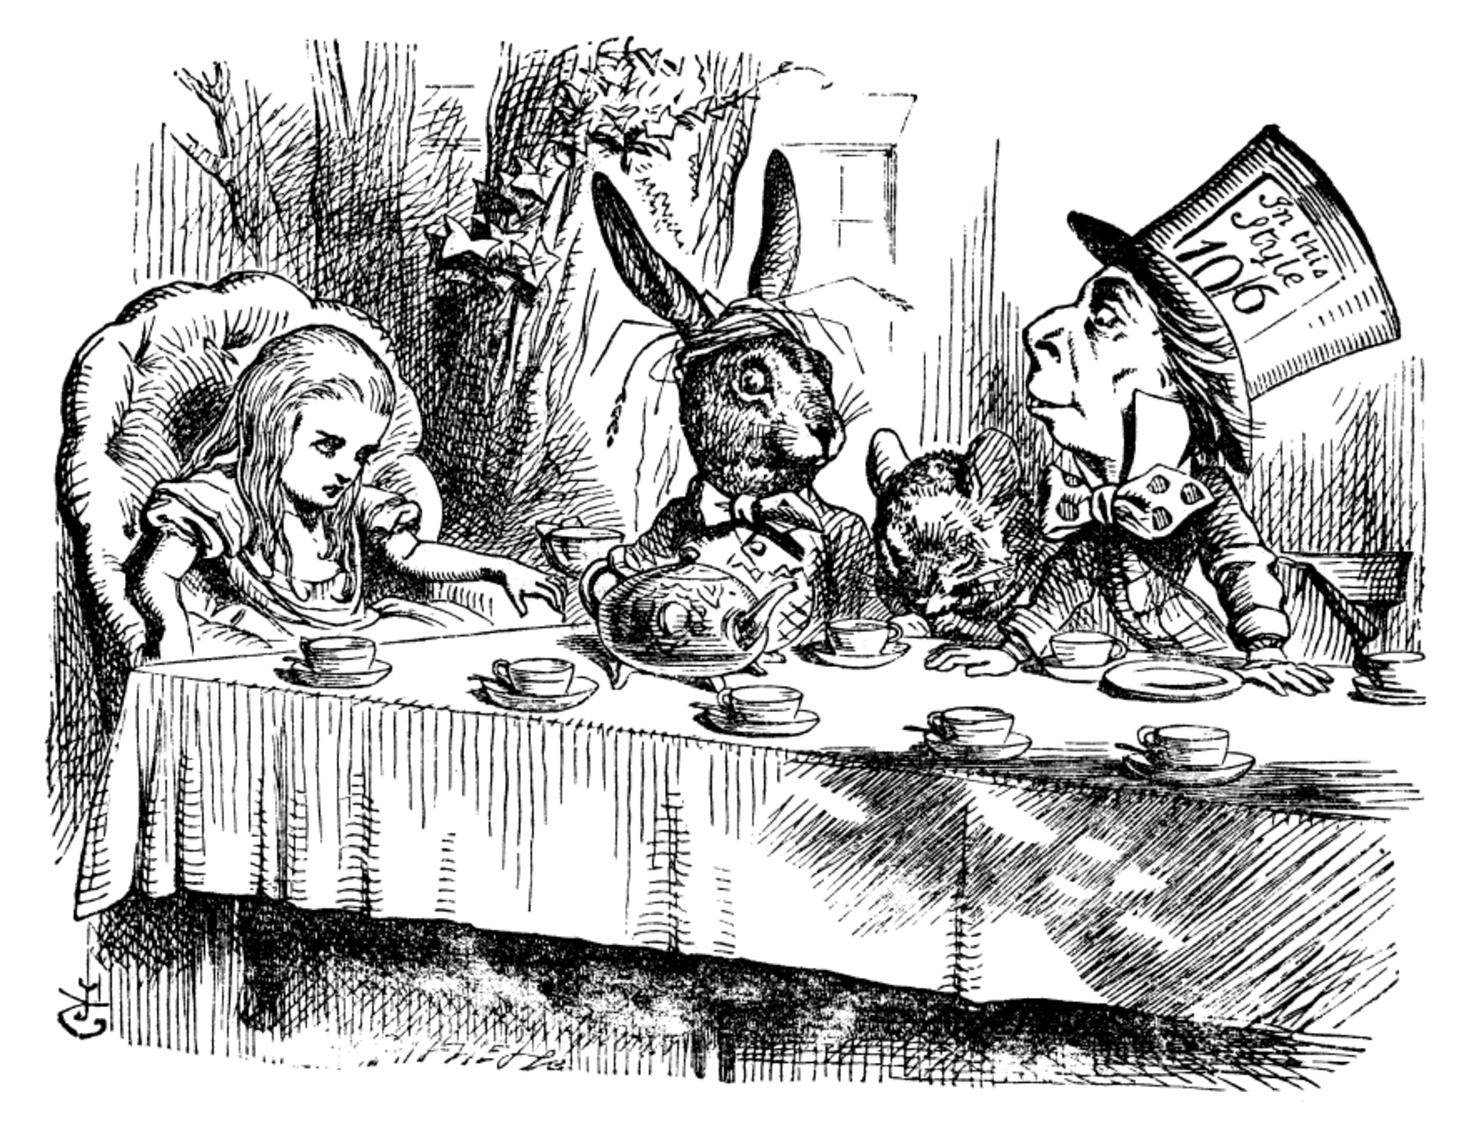
\includegraphics[width=0.85\textwidth]{alice-mad-tea-party}
    \caption{The Mad Hatter's Tea Party, from Alice's Adventures in Wonderland 
        by \citet{alice}. Illustration by John Tenniel 
        (1820-1914).}\label{fig:teaparty}
\end{figure}

\begin{table}[t!]\centering
%j.rnd.4x5.train.csv => instance problem.1
\caption{Example of $4\times5$ \JSP}\label{tbl:example}
\begin{tabular}{lc|ccccc|ccccc} \toprule
Guest & \multicolumn{1}{c}{Job} & \multicolumn{5}{c}{Machine ordering 
$\vsigma$} & \multicolumn{5}{c}{Processing times $\vec{p}$} \\ \midrule
%0 16 1 5 2 10 3 15 4 10 
Alice & \ref{guest:alice} & \st{1} & \st{2} & \st{3} & \st{4} & 
\st{5} & 
\st{26} & \st{25} & \st{40} & \st{15} & \st{42} \\
%0 18 1 16 2 36 3 68 4 44 
March Hare & \ref{guest:marchhare} & \st{1} & \textbf{2} & 3 & 4 & 5 & 
\st{18} & \textbf{86} & 86 & 68 & 84 \\
%4 20 3 9 2 3 1 33 0 96 
Dormouse & \ref{guest:dormouse} & \st{1} & \st{3} & \textbf{2} & 4 & 5 
& 
\st{20} & \textbf{59} & \st{23} & 33 & 96 \\
%4 40 3 7 1 15 5 13 2 80 
Mad Hatter & \ref{guest:madhatter} & \st{4} & \st{3} & \textbf{1} & 5 & 
2 & \textbf{40} & 47 & \st{55} & \st{13} & 99 
\\
\bottomrule
\end{tabular}
\end{table}

Unfortunately, Alice can't stay long. She must leave as soon as possible to 
play croquet with the Red Queen, 
and she mustn't be late for that very important date. Otherwise, it's off with 
someone's head! However, Alice, had a proper upbringing and won't leave the 
table until everyone has finished their tasks. 
How should the guests go about their tea-party, in order for Alice to be 
on-time?

The problem faced by Alice and her new friends is in what order should they 
rotate their tasks between themselves so that they all finish as soon as 
possible? This can be considered as is a typical four-job and five-machine 
\jsp, where
\begin{enumerate*}[label={{}}]
    \item our guests are the jobs
    \item their tasks are the machines
    \item our objective is to minimise $C_{\max}$, i.e., when Alice can 
    leave
\end{enumerate*}

Let's assume we've come to the party, after 10 operations have already been 
made (i.e. strikeout entries in \cref{tbl:example}), by using the following 
job sequence,\footnote{In fact this is the sequence resulting from 10 
    dispatches following the SPT-rule, to be defined shortly.}
\begin{equation}
\vchi = \left\{ \chi_i \right\}_{i=1}^{k-1} \label{eq:vchi:example}
= \left\{ J_4,J_2,J_3,J_3,J_1,J_1,J_1,J_1,J_1,J_4 \right\}
\end{equation}
hence currently, at step $k=11$, the job-list is 
$\mathcal{L}^{(k)}=\{J_2,J_3,J_4\}$ indicating the 3 potential\footnote{
    Alice is quite anxious to leave, so she has already completed everything, 
    and therefore \ref{guest:alice}$\notin\mathcal{L}^{(11)}$.} 
jobs (i.e. denoted in bold in \cref{tbl:example}) to be dispatched, i.e., 
$\chi_k\in\mathcal{L}^{(k)}$.

\tikzstyle{vertex}=[circle,fill=black!15,minimum size=20pt,inner sep=0pt]
\tikzstyle{completed vertex} = [vertex, fill=red!24]
\tikzstyle{possible vertex} = [vertex, fill=black!25]
\tikzstyle{edge} = [draw,thick,->,black!20]
\tikzstyle{proc} = [font=\small, below]
\tikzstyle{completed edge} = [draw,line width=2pt,->,red!50]
\tikzstyle{possible edge} = [draw,line width=4pt,->,black!20]
\tikzstyle{job line} = [line width=4mm,join=round]
\usetikzlibrary{backgrounds}

\begin{figure}[p]\centering
    \subcaptionbox{$k=0$\label{fig:example:graph:empty}}{
    \begin{tikzpicture}[scale=1.3, auto, swap]
    % Draw the network
    % First we draw the jobs
    \node at (-1,0) [fill=set1red] {$J_1$};
    \node at (-1,1) [fill=set1blue] {$J_2$};
    \node at (-1,2) [fill=set1green] {$J_3$};
    \node at (-1,3) [fill=set1purple] {$J_4$};
    % Second draw the machines / vertices    
    \foreach \pos/\name/\mac/\proc in {{(0,1.5)/Source}}
    \node[completed vertex] (\name) at \pos {$\mac$};
    \foreach \pos/\name/\mac/\proc in {{(6,1.5)/Sink},
        {(2,0)/J1M2/M_2/25},{(3,0)/J1M3/M_3/40},{(4,0)/J1M4/M_4/15},{(5,0)/J1M5/M_5/42},
        {(2,1)/J2M2/M_2/86},{(3,1)/J2M3/M_3/86},{(4,1)/J2M4/M_4/68},{(5,1)/J2M5/M_5/84},
        {(2,2)/J3M3/M_3/23},{(3,2)/J3M2/M_2/59},{(4,2)/J3M4/M_4/33},{(5,2)/J3M5/M_5/96},
        {(2,3)/J4M3/M_3/55},{(3,3)/J4M1/M_1/40},{(4,3)/J4M5/M_5/99},{(5,3)/J4M2/M_2/47}}
    \node[vertex] (\name) at \pos {$\mac$};
    \foreach \pos/\name/\mac/\proc in {
        {(1,0)/J1M1/M_1/26},{(1,1)/J2M1/M_1/18},{(1,2)/J3M1/M_1/20},{(1,3)/J4M4/M_4/13}}
    \node[possible vertex] (\name) at \pos {$\mac$};
    % Connect vertices with edges 
    \foreach \source/ \dest in {
        J1M1/J1M2,J1M2/J1M3,J1M3/J1M4,J1M4/J1M5,J1M5/Sink,
        J2M1/J2M2,J2M2/J2M3,J2M3/J2M4,J2M4/J2M5,J2M5/Sink,
        J3M1/J3M3,J3M3/J3M2,J3M2/J3M4,J3M4/J3M5,J3M5/Sink,
        J4M4/J4M3,J4M3/J4M1,J4M1/J4M5,J4M5/J4M2,J4M2/Sink}
    \path[edge] (\source) -- (\dest);
    \foreach \source/ \dest in {Source/J1M1,Source/J2M1,Source/J3M1,Source/J4M4}
    \path[possible edge] (\source) -- (\dest);
    % draw background for job's swimlane
    \begin{pgfonlayer}{background}
    \filldraw [job line,set1red!10]
    (J1M1.north -| J1M1.west) rectangle (J1M5.south -| J1M5.east);
    \filldraw [job line,set1blue!10]
    (J2M1.north -| J2M1.west) rectangle (J2M5.south -| J2M5.east);
    \filldraw [job line,set1green!10]
    (J3M1.north -| J3M1.west) rectangle (J3M5.south -| J3M5.east);
    \filldraw [job line,set1purple!10]
    (J4M4.north -| J4M4.west) rectangle (J4M2.south -| J4M2.east);
    \end{pgfonlayer}
\end{tikzpicture}
    }\\
    \subcaptionbox{$k=\nicefrac{K}{2}$\label{fig:example:graph:midway}}{
    \begin{tikzpicture}[scale=1.3, auto, swap]
    % Draw the network
    % First we draw the jobs
    \node at (-1,0) [fill=set1red] {$J_1$};
    \node at (-1,1) [fill=set1blue] {$J_2$};
    \node at (-1,2) [fill=set1green] {$J_3$};
    \node at (-1,3) [fill=set1purple] {$J_4$};
    % Second draw the machines / vertices    
    \foreach \pos/\name/\mac/\proc in {{(6,1.5)/Sink},
        {(3,1)/J2M3/M_3/86},{(4,1)/J2M4/M_4/68},{(5,1)/J2M5/M_5/84},
        {(4,2)/J3M4/M_4/33},{(5,2)/J3M5/M_5/96},
        {(4,3)/J4M5/M_5/99},{(5,3)/J4M2/M_2/47}}
    \node[vertex] (\name) at \pos {$\mac$};
    \foreach \pos/\name/\mac/\proc in {{(0,1.5)/Source}, 
        {(1,0)/J1M1/M_1/26},{(2,0)/J1M2/M_2/25},{(3,0)/J1M3/M_3/40},{(4,0)/J1M4/M_4/15},{(5,0)/J1M5/M_5/42},
        {(1,1)/J2M1/M_1/18},
        {(1,2)/J3M1/M_1/20},{(2,2)/J3M3/M_3/23},
        {(1,3)/J4M4/M_4/13},{(2,3)/J4M3/M_3/55}}
    \node[completed vertex] (\name) at \pos {$\mac$};
    \foreach \pos/\name/\mac/\proc in {
    {(2,1)/J2M2/M_2/86},{(3,2)/J3M2/M_2/59},{(3,3)/J4M1/M_1/40}}
    \node[possible vertex] (\name) at \pos {$\mac$};
    % Selected trajectory
    \path[possible edge] (J4M3) to[bend left] (J2M2);
    \path[possible edge] (J4M3) to (J3M2);
    \path[possible edge] (J4M3) to (J4M1);
    \path[completed edge] (J4M4) to[bend right] (J2M1);
    \path[completed edge] (J1M5) to[bend right=15] (J4M3);
    \foreach \source/ \dest in {
        Source/J4M4, J2M1/J3M1, J3M1/J3M3, J3M3/J1M1, J1M1/J1M2, 
        J1M2/J1M3, J1M3/J1M4, J1M4/J1M5} 
    \path[completed edge] (\source) -- (\dest);
    % Connect vertices with edges 
    \foreach \source/ \dest in {
        J2M2/J2M3,J2M3/J2M4,J2M4/J2M5,J2M5/Sink,
        J3M2/J3M4,J3M4/J3M5,J3M5/Sink,
        J4M1/J4M5,J4M5/J4M2,J4M2/Sink}
    \path[edge] (\source) -- (\dest);
    % draw background for job's swimlane
    \begin{pgfonlayer}{background}
    \filldraw [job line,set1red!10]
    (J1M1.north -| J1M1.west) rectangle (J1M5.south -| J1M5.east);
    \filldraw [job line,set1blue!10]
    (J2M1.north -| J2M1.west) rectangle (J2M5.south -| J2M5.east);
    \filldraw [job line,set1green!10]
    (J3M1.north -| J3M1.west) rectangle (J3M5.south -| J3M5.east);
    \filldraw [job line,set1purple!10]
    (J4M4.north -| J4M4.west) rectangle (J4M2.south -| J4M2.east);
    \end{pgfonlayer}
    \end{tikzpicture}
    
    }\\
    \subcaptionbox{$k=K$\label{fig:example:graph:final}}{
    \begin{tikzpicture}[scale=1.3, auto, swap]
    % Draw the network
    % First we draw the jobs
    \node at (-1,0) [fill=set1red] {$J_1$};
    \node at (-1,1) [fill=set1blue] {$J_2$};
    \node at (-1,2) [fill=set1green] {$J_3$};
    \node at (-1,3) [fill=set1purple] {$J_4$};
    % Second draw the machines / vertices
    \foreach \pos/\name/\mac/\proc in {{(0,1.5)/Source},{(6,1.5)/Sink},
        {(1,0)/J1M1/M_1/26},{(2,0)/J1M2/M_2/25},{(3,0)/J1M3/M_3/40},{(4,0)/J1M4/M_4/15},{(5,0)/J1M5/M_5/42},
        {(1,1)/J2M1/M_1/18},{(2,1)/J2M2/M_2/86},{(3,1)/J2M3/M_3/86},{(4,1)/J2M4/M_4/68},{(5,1)/J2M5/M_5/84},
        {(1,2)/J3M1/M_1/20},{(2,2)/J3M3/M_3/23},{(3,2)/J3M2/M_2/59},{(4,2)/J3M4/M_4/33},{(5,2)/J3M5/M_5/96},
        {(1,3)/J4M4/M_4/13},{(2,3)/J4M3/M_3/55},{(3,3)/J4M1/M_1/40},{(4,3)/J4M5/M_5/99},{(5,3)/J4M2/M_2/47}}
    \node[completed vertex] (\name) at \pos {$\mac$};
    % Selected trajectory
    \path[completed edge] (J4M4) to[bend right] (J2M1);
    \path[completed edge] (J1M5) to[bend left=17] (J4M3);
    \foreach \source/ \dest in {
        Source/J4M4, J2M1/J3M1, J3M1/J3M3, J3M3/J1M1, J1M1/J1M2, J1M2/J1M3, 
        J1M3/J1M4, J1M4/J1M5, J4M3/J4M1, J4M1/J3M2, J3M2/J3M4, J3M4/J2M2, 
        J2M2/J2M3, J2M3/J2M4, J2M4/J2M5, J2M5/J3M5, J3M5/J4M5, J4M5/J4M2, 
        J4M2/Sink} 
    \path[completed edge] (\source) -- (\dest);
    % draw background for job's swimlane
    \begin{pgfonlayer}{background}
    \filldraw [job line,set1red!10]
    (J1M1.north -| J1M1.west) rectangle (J1M5.south -| J1M5.east);
    \filldraw [job line,set1blue!10]
    (J2M1.north -| J2M1.west) rectangle (J2M5.south -| J2M5.east);
    \filldraw [job line,set1green!10]
    (J3M1.north -| J3M1.west) rectangle (J3M5.south -| J3M5.east);
    \filldraw [job line,set1purple!10]
    (J4M4.north -| J4M4.west) rectangle (J4M2.south -| J4M2.east);
    \end{pgfonlayer}
    \end{tikzpicture}
    
    }
    \caption[Graph representation for \JSP]{Graph representation of a 
    $4\times5$ \jsp, where pink vertices are completed tasks, and grey are 
    unassigned. Moreover, grey arrows point to the operations that are 
    next on the job-list, $\mathcal{L}^{(k+1)}$, and pink arrows 
    (traversing from source towards sink) yield the sequence of operations for 
    the schedule, i.e., $\vchi$.}\label{fig:example:graph}
\end{figure}


This is a very compact form for the current partial solution, it's easiest to 
comprehend it via disjunctive graph \citep{roy64} to model the work-flow of 
tasks to be scheduled.
Let's encode
\begin{enumerate*}
    \item the operations as vertices
    \item horizontally aligning them w.r.t. each job $J_j$
    \item connect vertices with directed edges according the 
    \cref{eq:permutation}
    \item by introducing dummy vertices before and after, then the goal is to 
    visit each vertex exactly once, or \emph{Hamiltonian} path: starting at the 
    `source'  (i.e. empty schedule), and finishing at the sink (i.e. complete 
    schedule)
\end{enumerate*}
The path gives the prescription of the order in which the jobs rotate 
between machines. 
\Cref{fig:example:graph} depicts the path generation at the beginning, midway, 
and final stages for our Tea Party. 
\begin{enumerate*}
    \item gray vertices are operations that haven't yet been dispatched
    \item pink vertices are the ones that correspond to $\vchi$
    \item pink directed edges indicate the current partial Hamiltonian path
\end{enumerate*}
%Note, \cref{fig:example:graph:midway} corresponds to \cref{eq:vchi:example}.

\begin{figure}\centering
    \includegraphics[width=0.9\textwidth]{{example.gantt}.pdf}
    \caption[Gantt chart of a partial \JSP\ schedule]{Gantt chart of a partial 
        \JSP\ schedule after 10 dispatches: Solid and dashed boxes represent 
        $\vchi$ and $\mathcal{L}^{(11)}$, respectively. Current $C_{\max}$ 
        denoted 
        as dotted line.}
    \label{fig:example:midway}
\end{figure}

Now we're interested to know when each guest should start their task, 
i.e., the project schedule. \Cref{fig:example:midway} illustrates the 
temporal partial schedule (or $k$-solution) of \cref{eq:vchi:example} as a 
Gantt-chart
\begin{enumerate*}
    \item numbers in the boxes represent the job identification $j$
    \item the width of the box illustrates the processing times for a given job 
    for a particular machine $M_a$ (on the vertical axis)
    \item the dashed boxes represent the resulting $(k+1)$-solution for when a 
    particular job is scheduled next 
    \item the current $C_{\max}$ is denoted with a dotted line    
\end{enumerate*}
Note, the disjunctive graph from \cref{fig:example:graph:midway} gives the 
schedule in \cref{fig:example:midway}.

If the job with the shortest processing time were to be scheduled next, i.e., 
applying SPT-rule, then $J_4$ would be dispatched. Similarly, for  LPT-rule 
(largest processing time) then $J_2$ would be dispatched. 
Other DRs use features not directly observable from looking at the $k$-solution 
(but easy to keep record of), e.g., by assigning jobs 
with most or least total processing time remaining, i.e., MWR and LWR 
heuristics, who would yield $J_2$ and $J_4$, respectively.

\section{Single priority based \dr s}\label{sec:SDR}

A \emph{\sdr} (SDR) is a function of attributes, or features, of the jobs 
and/or machines of the schedule. The features can be constant or vary 
throughout the scheduling process. 
For instance, priority may depend on job processing attributes, such as 
which job has, 
\begin{description}
    \item[Shortest immediate processing time (SPT)] \hfill \\
    greedy approach to finish shortest tasks first,  
    \item[Longest immediate processing time (LPT)] \hfill \\
    greedy approach to finish largest tasks first, 
    \item[Least work remaining (LWR)] \hfill \\
    whose intention is to complete jobs advanced in their pro\-gress, i.e., 
    minimising $\mathcal{L}$,
    \item[Most work remaining (MWR)] \hfill \\
    whose intention is to accelerate the processing of jobs that require a 
    great deal of work, yielding a balanced progress for all jobs during 
    dispatching. However, in-process inventory can be high.
\end{description}
These rules are the ones most commonly applied in the literature due to their 
simplicity and surprising efficiency. %\citep[cf.][]{Haupt89,Panwalkar77}
Therefore, they will be referenced throughout the dissertation. 
However, there are many more available, e.g., randomly selecting an operation 
with equal possibility (RND); minimum slack time (MST); smallest slack per 
operation (S/OP); and using the aforementioned dispatching rules with 
predetermined weights. 
A survey of more than 100 of such rules are presented in \citet{Panwalkar77}. 
However, the reader is referred to an in-depth survey for SDRs by 
\citet{Haupt89}. 


%Haupt89:
%Among the rules with job processing information, SPT is the most known, the 
%most applied, and yet one of the most efficient rules. In line with LPT, it 
%requires the lowest information amount, since only operation data (not job 
%data) from the local queue (not from other queues) are needed.
%LWR give preference to jobs the work completed of which is rather advanced. 
%Thus, they can be regarded as value-oriented rules selecting jobs with a high 
%fraction of their value added or cumulative value to their total value.
% The intent of MWR is to speed up jobs with large processing work resulting in 
%a well-balanced work progress of all jobs, at the expense of a high volume of 
%in-process inventory, while LWR tend to reduce the number of jobs in the shop.

To summarise, SDRs assign an index to each job of the job-list waiting to be 
scheduled, and are generally only based on few features and simple mathematical 
operations. 
Continuing with the example from \cref{sec:jsp:example}, the final schedules 
for these main SDRs (and a possible optimal schedule for reference) are 
depicted in \cref{fig:example:SDRs}. As we can see, MWR would have  been 
the best strategy for Alice and company, since it has the makespan closest to 
the optimum. 

\begin{figure}[t]
    \includegraphics[width=\textwidth]{{example.gantt.SDRs}.pdf}
    \caption{SDRs applied to the Tea-party example in \cref{sec:jsp:example}. 
        A possible optimal solution is shown in the lower right 
        corner as a reference.}
    \label{fig:example:SDRs}
\end{figure}

\section{Features for \jsp}\label{sec:features}
A DR may need to perform a one-step look-ahead, and observe features of the 
partial schedule to make a decision. 
For example by observing the resulting temporal makespan. 
These emanated observed features are sometimes referred to as an 
\emph{after-state} or \emph{post-decision state}. 
A $k$-solution is denoted $\vchi^j$ where $J_j$ is the latest dispatch, i.e., 
$\chi_k=J_j$, and its resulting features is denoted, 
\begin{equation}\label{eq:postdecision}
\vphi^j:=\vphi(\vchi^j).
\end{equation}

Features are used to grasp the essence of the current state of the schedule. 
Temporal scheduling features applied in this dissertation are given in 
\cref{tbl:features}. 


The features of particular interest were obtained from inspecting the 
aforementioned SDRs from \cref{sec:SDR}: namely \phiproc\ and \phijobWrm. 
Moreover, \phiJobRelated\ and \phiMacRelated\ are job-related and 
machine-related attributes of the current schedule, respectively. 

Some features are directly observed from the $k$-solution, such as the job- 
and machine-related features, namely, \phiLocalRelated\ and they are only based 
on the current step of the schedule, 
i.e., schedule's \emph{local features}, and might not give an accurate 
indication of how it will effect the schedule in the long run. Therefore, a set 
of features are needed to estimate the schedule's overall performance, referred 
to as its \emph{global features}. 

The approach here is to use well known SDRs, \phiSDRRelated, as a benchmark by 
retrieving what would the resulting $C_{\max}$ be given if that SDR would 
be implemented from that point forward. 
Moreover, random completion of the $k$-solution are implemented, 
here \phiRNDRelated\ corresponds to statistics from 100 random roll-outs, which 
can be used to identify which features $\vphi$ are promising on a long-term 
basis. 
\emph{Roll-out algorithms} \citep{Bertsekas97}, also known as \emph{Pilot 
    Method} \citep{Duin99}, for combinatorial optimisation aim to improve 
performance by sequential application of a pilot heuristic, which completes the 
remaining $K-k$ steps. Roll-outs for \JSP\ have been conducted by 
\citet{Ru12}. Continuing with that work, \citet{Geirsson2012} compares several 
pilot heuristics, e.g., \emph{Randomly Chosen Dispatch Rules} which is similar 
to \phiSDRRelated\ (but here one roll-out per fixed SDR). 
The motivation being, that a SDR-based roll-out are of higher quality than 
random ones, requiring less computational budget. 
However, \citeauthor{Geirsson2012} notes that performance w.r.t. traditional 
random roll-outs is statistically insignificant, and not worth the overhead of 
implementing various SDRs beforehand. 

\citeauthor{Geirsson2012} reworks the roll-out algorithm as an 
$\abs{\mathcal{L}}$-armed bandit,\footnote{In probability theory, the
    multi-armed bandit problem \citep{badit:book} describes a gambler at a row 
    of slot machines, who has to decide which machines to play, i.e., pull its 
    lever, in  order to maximise his rewards, that are specific to each 
    machine. The gambler also has to decide how many times to play each machine 
    and in which order to play them. The gambler's actions are referred to as 
    \emph{pilot-heuristic}.} 
i.e., each job of the job-list are the levers. Since the best job, $j^*$, to 
dispatch at step $k$, is not known beforehand, therefore all available jobs are 
evaluated, using roll-outs. 
As a result, using the features \phiRNDRelated, the weights $\vec{w}$ yield the 
deterministic pilot heuristic. Although in \citeauthor{Geirsson2012}'s work, 
other statistics are used for guidance, e.g., quartile and octile. 

It's noted, that the roll-outs considered in this dissertation, are with a very 
frugal budget, only 100 roll-outs per lever is considered -- all evenly 
distributed between levers. But using the multi-armed bandit paradigm, it's 
possible to allocate roll-outs originating from the job-list with bias towards 
more promising levers.

\begin{table} \centering 
    \caption[Feature space $\mathcal{F}$ for \JSP]{Feature space $\mathcal{F}$ 
        for \JSP\ where job $J_j$ on machine $M_a$ given the resulting temporal 
        schedule after dispatching $(j,a)$.}
    \label{tbl:features}
     {\footnotesize
 \centering
 \renewcommand{\arraystretch}{1.5}
  \begin{tabular}{clll}
	\toprule
  $\vphi$ & Feature description   & Mathematical formulation & Shorthand  \\ 
  %\hline  \multicolumn{4}{c}{\textbf{Local features}}  \\
  \midrule
  \multicolumn{4}{c}{\textbf{job related}}\\
  \phiproc         & job processing time                       & $p_{ja}$   & 
  proc         \\
  \phistartTime    & job start-time                            & $x_s(j,a)$ & 
  startTime    \\
  \phiendTime      & job end-time                              & $x_e(j,a)$ &
  endTime      \\
  \phiarrivalTime  & job arrival time                          & $x_e(j,a-1)$&
  arrival      \\ 
  \phiwait         & time job had to wait                      & 
  $x_s(j,a)-x_e(j,a-1)$ & 
  wait         \\   
  \phijobTotProcTime    & total processing time for job             & 
  $\sum_{a\in \mathcal{M}}p_{ja}$ & 
  jobTotProcTime \\
  \phijobWrm       & total work remaining for job              & 
  $\sum_{a'\in\mathcal{M}\setminus \mathcal{M}_{j}}p_{ja'}$ & 
  jobWrm       \\
  \phijobOps       & number of assigned operations for job     & 
  $|\mathcal{M}_j|$ & 
  jobOps       \\ 
  \midrule
  \multicolumn{4}{c}{\textbf{machine related}}\\
  \phimacFree      & when machine is next free                 & 
  $\max_{j'\in \mathcal{J}_a} \{x_e(j',a)\}$ &
  macFree      \\
  \phimacTotProcTime    & total processing time for machine    & 
  $\sum_{j\in \mathcal{J}}p_{ja}$ & 
  macTotProcTime \\
  \phimacWrm       & total work remaining for machine          & 
  $\sum_{j'\in\mathcal{J}\setminus \mathcal{J}_{a}}p_{j'a}$ &  
  macWrm       \\
  \phimacOps       & number of assigned operations for machine & 
  $|\mathcal{J}_a|$ & 
  macOps       \\
  \phireducedSlack & change in idle time by assignment         & 
  $\Delta s(a,j)$ &
  reducedSlack \\
  \phimacSlack        & total idle time for machine               & 
  $\sum_{j'\in \mathcal{J}_a}s(a,j')$ &
  macSlack        \\
  \phiallSlack   & total idle time for all machines          & $\sum_{a'\in 
    \mathcal{M}}\sum_{j'\in \mathcal{J}_{a'}}s(a',j')$                    & 
  allSlack   \\
  \phimakespan     & current makespan                          &
  $\max_{(j',a')\in \mathcal{J} \times \mathcal{M}_{j'}}\{x_f(j',a')\}$ & 
  makespan     \\
  \midrule
  \multicolumn{4}{c}{\textbf{final makespan related}}\\
  \phiSPT & final makespan using SPT & $ C_{\max}^{\SPT}$ & SPT \\
  \phiLPT & final makespan using LPT & $ C_{\max}^{\LPT}$ & LPT \\
  \phiLWR & final makespan using LWR & $ C_{\max}^{\LWR}$ & LWR \\
  \phiMWR & final makespan using MWR & $ C_{\max}^{\MWR}$ & MWR \\
  $\phiRND$ & final makespans using 100 random rollouts & $ 
  \{C_{\max}^{\RND}\}_{i=1}^{100}$ & \\  
  \phiRNDmean & mean for $\phiRND$ & $\Exp{\phiRND}$ & RNDmean \\  
  \phiRNDstd & standard deviation for $\phiRND$ & 
  $\sqrt{\Exp{\phiRND^2}-\Exp{\phiRND}^2}$ &
  RNDstd \\
  \phiRNDmin & minimum value for $\phiRND$ & $\min\{\phiRND\}$ & RNDmin \\  
  \phiRNDmax & maximum value for $\phiRND$ & $\max\{\phiRND\}$ & RNDmax \\  
  \bottomrule
  \end{tabular}
}
 %Feature description for job $J_j$ on machine $M_a$ given current temporal schedule, where the set of jobs already dispatched are $J\subset\mathcal{J}$ on corresponding set of machines $\mathcal{M}_j\subset\mathcal{M}$

\end{table}

\section{Composite dispatching rules}\label{sec:CDR}

Priority \dr s were originally introduced in \citet{Giffler60} to resolve 
conflicts of the job-list, and have made great headway since. 
They are especially attractive since they are relatively simple to 
implement, fast and find good schedules. In addition, they are easy 
to interpret, which makes them desirable for the end-user (i.e. shop floor 
operators). 
However, they can also fail unpredictably. 
\citet{Jayamohan04} showed that a careful combination of \dr s can 
perform significantly better. These are referred to as \emph{composite 
dispatching rules} (CDR), where the priority ranking is an expression of 
several DRs. 

For instance, optimising $J1||L_{\max}$ \cite[see. chapter 14.2]{Pinedo08}, one 
can combine SDRs that are optimal for a different criteria of problem 
instances, which complement each other as a CDR, e.g., combining the SDRs 
\begin{enumerate*}[after={{}}]
    \item WSPT \footnote{WSPT is optimal when all release dates and due dates 
        are zero.} (SPT weighted w.r.t. $\mathcal{J}$)
    \item minimum slack first (MS),\footnote{MS is optimal when all due dates 
        are sufficiently loose and spread out.} 
\end{enumerate*}
yields the CDR \emph{Apparent Tardiness Cost}, which can work well on a 
broader set of problem instances than the original SDRs by themselves.

%\subsection*{Mathematical formulation of CDRs}

CDRs can deal with a greater number of more complicated functions constructed 
from the schedules attributes. In short, a CDR is a combination of several DRs. 
For instance let $\pi$ be a CDR comprised of $d$ DRs, then the index $I$ for 
$J_j\in\mathcal{L}^{(k)}$ using $\pi$ is, 
\begin{equation}\label{eq:CDR}
I_j^{\pi} = \sum_{i=1}^d w_i \pi_i(\vchi^j) 
\end{equation}
where $w_i>0$ and $\sum_{i=0}^d w_i = 1$, then $w_i$ gives the \emph{weight} of 
the influence of $\pi_i$ (which could be a SDR or another CDR) to $\pi$. Note, 
each $\pi_i$ is function of $J_j$'s attributes from the $k$-solution $\vchi^j$.

The \cdr\ presented in \cref{eq:CDR} can be considered as a special case of a 
the following general linear value function,
\begin{equation}\label{eq:CDR:feat}
\pi(\vchi^j) = \sum_{i=1}^d w_i \phi_i(\vchi^j)
\stackrel{\eqref{eq:postdecision}}{=} \inner{\vec{w}}{\vphi^j}.
\end{equation}
when $\pi_i(\cdot)=\phi_i(\cdot)$, i.e., a composite function of the features 
from \cref{tbl:features}. 

Finally, the job to be dispatched, $J_{j^*}$, corresponds to the one with the 
highest value, i.e.,
\begin{equation}
J_{j^*}=\argmax_{J_j\in \mathcal{L}}\; \pi(\vphi^j)
\end{equation}

Since we're using a feature space based on job-attributes, then it's trivial to 
interpret \cref{eq:CDR:feat} as the SDRs from \cref{sec:SDR}. 
Then for $i\in\{1,\ldots,d\}$, they're simply,

\begin{subequations}
    \begin{IEEEeqnarray}{s"rCl} 
        SPT:& w_i&=&\bigg\{ \begin{array}{rl}-1&\text{if 
            }i=1\\0&\text{otherwise}\end{array}  \\
        LPT:& w_i&=&\bigg\{ \begin{array}{rl} 1&\text{if 
            }i=1\\0&\text{otherwise}\end{array}  \\
        MWR:& w_i&=&\bigg\{ \begin{array}{rl} 1&\text{if 
            }i=7\\0&\text{otherwise}\end{array}  \\
        LWR:& w_i&=&\bigg\{ \begin{array}{rl}-1&\text{if 
            }i=7\\0&\text{otherwise}\end{array} \label{pref:SDR}
    \end{IEEEeqnarray} 
\end{subequations}


\subsection*{Automated discovery of CDRs}
Generally the weights $\vec{w}$ in \cref{eq:CDR:feat} are chosen by the 
algorithm designer a priori. 
A more sophisticated approach would have the algorithm discover these 
weights autonomously. For instance via preference-based 
imitation learning or evolutionary search, to be discussed in 
\cref{ch:prefmodels} and \cref{ch:esmodels}, respectively.

\citet{Monch13} stress the importance of automated discovery of DRs and named 
several successful such implementations in the field of semiconductor wafer 
fabrication facilities. 
However, \citeauthor{Monch13} note that this sort of investigation is still in 
its infancy and subject for future research.

\clearpage
A recent editorial of the state-of-the-art approaches in advanced dispatching 
rules for large-scale manufacturing systems by \citet{Chen13} points out that:
\begin{quote}
    [..] most traditional dispatching rules are based on historical data. With 
    the emergence of data mining and on-line analytic processing, dispatching 
    rules can now take predictive information into account.
\end{quote}
implying that there has not been much automation in the process of discovering 
new dispatching rules, which is the ultimate goal of this dissertation, i.e., 
automate creation of optimisation heuristics for scheduling. 

With meta heuristics one can use existing DRs and use for example 
{portfolio-based algorithm selection} either based 
on a single instance \citep{Rice76,Gomes01} or class of instances \citep{Xu07} 
to determine which DR to choose from. 
Instead of optimising which algorithm to use under what data distributions, 
such as the case of portfolio algorithms, the approach taken in this 
dissertation is more similar to that of \emph{meta learning} \citep{Vilalta02}, 
which is the study of how learning algorithms can be improved, i.e., exploiting 
their strengths and remedy their failings, in order for a better algorithm 
design. Thus, creating an adaptable learning algorithm that dynamically finds 
the appropriate dispatching rule  to the data distribution at hand. 

\citet{Kalyanakrishnan11} point out that meta learning can be very fruitful in 
reinforcement learning, and in their experiments they discovered some key 
discriminants between competing algorithms for their particular problem 
instances, which provided them with a hybrid algorithm which combines the 
strengths of the algorithms.

\citet{Nguyen13} proposed a novel {iterative dispatching rules} for \JSP\ 
which learns from completed schedules in order to iteratively improve new ones. 
At each dispatching step, the method can utilise the current feature space to 
`correctify' some possible `bad' dispatch made previously (sort of reverse 
lookahead). Their method is straightforward, and thus easy to implement and 
more importantly, computationally inexpensive, although \citeauthor{Nguyen13} 
stress that there still remains room for improvement. 

\citet{Korytkowski13} implemented {ant colony optimisation} to select the 
best DR from a selection of 9 DRs for \JSP\ and their experiments showed 
that the choice of DR do affect the results and that for all performance 
measures considered it was better to have all of the DRs to choose from rather 
than just a single DR at a time. 

Similarly, \citet{Lu13} investigate 11 SDRs for \JSP\ to create a pool of 
33 CDRs that strongly outperformed the ones they were based on. The CDRs were 
created with {multi-contextual functions} based either on machine idle time 
or job waiting time (similar to \phiwait\ and \phimacSlack\ in 
\cref{tbl:features}), creating CDRs thate are a combination of those 
two key features of the schedule and then the basic DRs. However, there are no 
combinations of the basic DR explored, only machine idle time and job waiting 
time.  

\citet{Yu13} used priority rules to combine 12 existing DRs from the 
literature, in their approach they had 48 priority rules combinations, 
yielding 48 different models to implement and test. This is a fairly 
ad-hoc solution and there is no guarantee the optimal combination of DRs is 
found. 

It is intuitive to get a boost in performance by introducing new CDRs, since 
where one DR might be failing, another could be excelling so combining them 
together should yield a better CDR. However, these aforementioned approaches 
introduce fairly ad-hoc solutions and there is no guarantee the optimal 
combination of \dr s were found.

\section{Rice's framework for \jsp}\label{sec:rice:jsp}
\citeauthor{Rice76}'s framework for algorithm selection (discussed in 
\cref{sec:rice}) has already been formulated for \jsp\ (cf. 
\citet{SmithMilesLion3,SmithMilesLion5} and \cref{InRu12}), as follows, 
\begin{description} 
    \item[Problem space] $\mathcal{P}$ is defined as the union of $N$ problem 
    instances consisting of processing time and ordering matrices, 
    $\vec{x}=(\vec{p},\vsigma)$, for $n$-jobs and $m$-machines, 
    \begin{equation} 
    \mathcal{P}=\condset{\vec{x}_i}{n\times m~}_{i=1}^{N}
    \end{equation}
    Problem generators for $\mathcal{P}$ are given in 
    \cref{ch:genprobleminstances}.
    \item[Feature space] $\mathcal{F}$ which was outlined in 
    \cref{sec:features}. Note, these are not the only possible set of features. 
    However, the local feature, \phiLocalRelated, are built on the work by 
    \cite{SmithMilesLion3} and \cref{InRu11a} and deemed successful in 
    capturing the essence of a \jsp\ data structure;
    \item[Algorithm space] $\mathcal{A}$ is simply the scheduling policies 
    under consideration, e.g., SDRs from \cref{sec:SDR},
    \begin{equation}
    \mathcal{A}=\left\{\text{SPT,~LPT,~LWR,~MWR,~RND,~}\dotsc\right\}.
    \end{equation} 
    \item[Performance space] $\mathcal{Y}$ is based on the resulting 
    $C_{\max}$, defined by \cref{eq:makespan}. The optimum makespan is denoted 
    $C_{\max}^{\pi_\star}$, i.e., following the expert policy $\pi_\star$, and 
    the makespan obtained from the scheduling policy $\pi\in\mathcal{A}$ under 
    inspection by $C_{\max}^{\pi}$. 
    Since the optimal makespan varies between problem instances the performance 
    measure is the following, 
    \begin{equation}\label{eq:rho}
    \rho=\frac{C_{\max}^{\pi}-C_{\max}^{\pi_\star}}{C_{\max}^{\pi_\star}}\cdot
    100\%
    \end{equation}
    which indicates the \namerho. Thus $\mathcal{Y}$ is given as, 
    \begin{equation}
    \mathcal{Y}=\left\{\rho_i\right\}_{i=1}^{N}
    \end{equation}
    \Cref{eq:rho} measures the discrepancy between predicted value and true 
    outcome, and is commonly referred to as a loss function, which we would 
    like to minimise for $\pi$.
\end{description}
The mapping $\Upsilon:\;\mathcal{A}\times\mathcal{F} \mapsto \mathcal{Y}$ is 
the step-by-step construction heuristic in \cref{pseudo:constructJSP}.